\documentclass[11pt]{article}

\usepackage[numbers,sort&compress]{natbib}  
%% Daniel added this, should help citations look nicer. You may need to delete temp files and rebuild the latex document from a clean start.

\newcommand{\daniel}[1]{{\textbf{{\small{\color{magenta}DL}: #1{\color{magenta}$\circ$}}}}} 
\newcommand{\owen}[1]{\textbf{{\small{\color{red}OK}: #1{\color{red}$\circ$}}}} 
\newcommand{\ed}[1]{\textbf{{\small{\color{blue}ED}: #1{\color{blue}$\circ$}}}}

%\renewcommand{\daniel}[1]{}
%\renewcommand{\owen}[1]{}
%\renewcommand{\ed}[1]{}


% Use utf-8 encoding for foreign characters
\usepackage[utf8]{inputenc}
\usepackage{url}
% Setup for fullpage use
\usepackage{fullpage}
\usepackage{color}
\usepackage{subfig}
\usepackage{hyperref}
\usepackage[noend]{algorithm2e}
\usepackage{algorithmic}

% Uncomment some of the following if you use the features
%
% Running Headers and footers
%\usepackage{fancyhdr}

% Multipart figures
%\usepackage{subfigure}

% More symbols
%\usepackage{amsmath}
%\usepackage{amssymb}
%\usepackage{latexsym}

% Surround parts of graphics with box
\usepackage{boxedminipage}

% Package for including code in the document
\usepackage{listings}

% If you want to generate a toc for each chapter (use with book)
\usepackage{minitoc}

% This is now the recommended way for checking for PDFLaTeX:
\usepackage{ifpdf}

%\newif\ifpdf
%\ifx\pdfoutput\undefined
%\pdffalse % we are not running PDFLaTeX
%\else
%\pdfoutput=1 % we are running PDFLaTeX
%\pdftrue
%\fi

% \ifpdf
\usepackage[pdftex]{graphicx}
% \else
% \usepackage{graphicx}
% \fi

\title{RMS and Backpropagation for Feedforward Neural Networks}
\author{Eduardo Gutarra}

% \date{2010--06--13}

\begin{document}
	
\ifpdf
\DeclareGraphicsExtensions{.pdf, .jpg, .tif}
\else
\DeclareGraphicsExtensions{.eps, .jpg}
\fi
	
\maketitle
	
\section{Introduction} % (fold)
\label{sec:introduction}

Artificial neural networks are computational models that mimic the architecture, structure and/or functional aspects of biological
neural networks such as the human brain. They are comprised of multiple processing elements called neurons which are interconnected
through links. Often, these links have weights associated to them called synaptic weights. These weights scale the signals received from
different neurons, allowing the network to process patterns and generate an output pattern. The synaptic weights are free parameters
that may be changed, allowing the neural network to change its behavior. In artificial neural networks, neurons are often grouped
together in layers or slabs and a neural network may be composed of 1 or more of these~\cite{skapura}. As an example, a feedforward
neural network is illustrated in Figure~\ref{fig:figures_ffwdnn}.

The overall behavior of the neural network is determined by the behavior of each individual neuron. Each neuron gathers input from the external environment or neighbohr neurons that are connected to it. The neuron then sums the modulated input and ...

Neural networks possess important advantages and capabilities as computational models. Among these include their ability to: solve
problems of nonlinear nature, perform input-output mapping through a learning process, adaptation to new situations, and their inherent
parallelism~\cite{Haykin:1994:NNC:541500}. One of the greatest advantages of using a neural network is that we do not program it with a
configuration to solve a problem. It is actually programmed to learn and adapt to solve a problem. Neural networks have two types of
learning supervised and unsupervised learning. Supervised learning consists in giving a network a set of points and allowing to correct
its prediction by giving it the expected output. Unsupervised learning is often used when the network cannot be provided with a target
output, and therefore works with evolutionary models.

Even though biological neurons are 6 orders of magnitude slower than the integrated circuits found in today's computer processors. They
work as a massively parallel system allowing efficient solutions to complex problems such as facial recognition. These problems are
still a challenge today for artificial neural networks. Today's artificial neural networks have been successfully applied in
applications such as: Function approximation or regression analysis and Classification, including pattern and sequence recognition among
others.

Our interest in this report is confined to a class of neural networks which emulate the process of learning. In this report we will
examine two different algorithms for training feedforward neural networks. One algorithm is the Back-propagation algorithm and the other
is the Root Mean Square (RMS) Minimization algorithm.

\begin{figure}[]
	\centering
		\subfloat[\label{fig:figures_ffwdnn} A feedforward neural network with labeled constituents]{	
				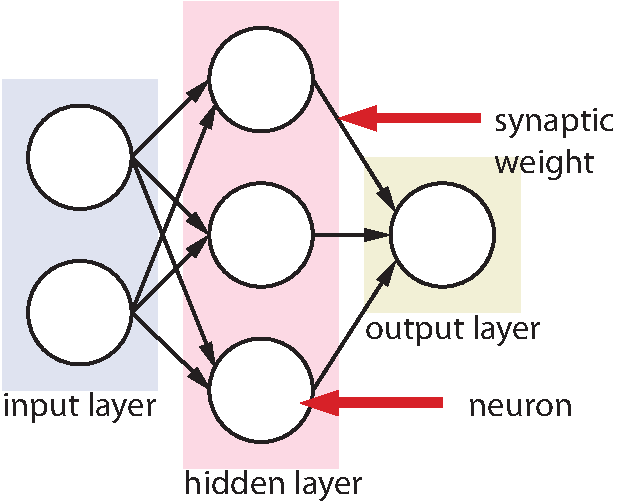
\includegraphics[height=0.30\columnwidth]{figures/ffwdnn.pdf}
		}
		\subfloat[\label{fig:figures_Neuron} A neuron and its constituents]{	
				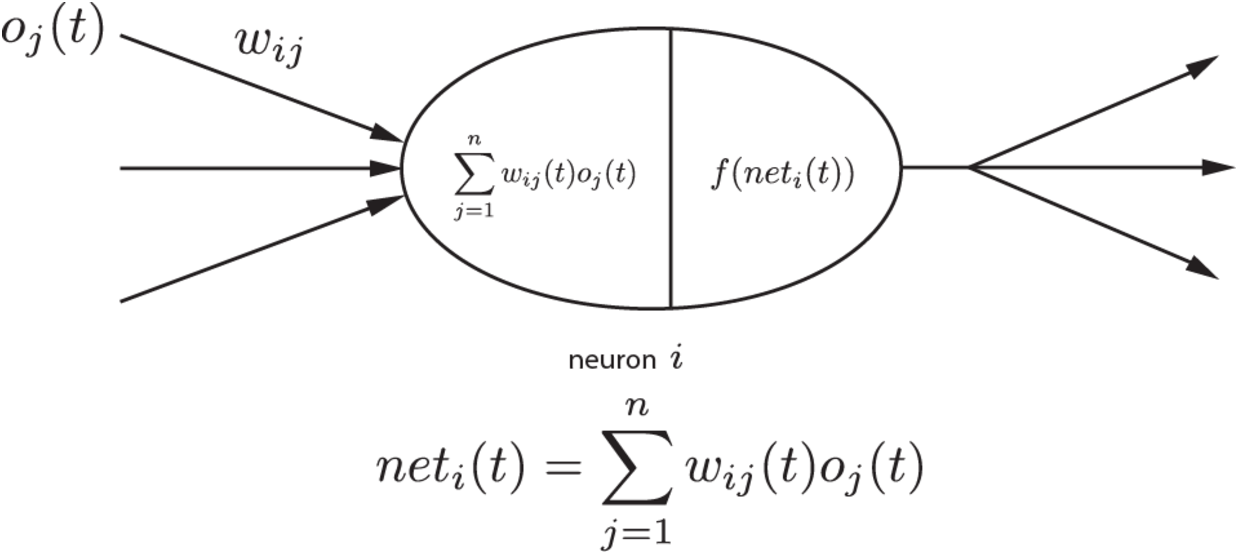
\includegraphics[height=0.25\columnwidth]{figures/Neuron.pdf}
		}
		\caption{feedforward neural network and its processing element the neuron}
	\label{fig:figures_ffwdnn_Neuron}	
\end{figure}

\section{Feedforward Neural Networks} % (fold)
\label{sec:feedforward_neural_networks}

In a feedforward neural network only neurons of adjacent layers are interconnected with synaptic weights. Each layer of the neural
network has connections to the next layer and there are no connections oriented backwards.

The feedforward neural network begins with an input layer which may be connected to a hidden layer or directly to an output layer. The
first layer is the input layer. It connects directly to the external environment and captures the input patterns presented to the
network. The last layer is the output layer which produces the output pattern to the external environment. All other layers are
considered hidden and may or may not be present.

The processing of a feedforward neural network begins when an external pattern made up of signals is captured by an input layer (see
Algorithm~\ref{alg:feedforward}).

\begin{algorithm}% [H]
\KwIn{Set of inputs from the environment}
\KwOut{Set of output values calculated by the feedforward neural network}
\SetLine
\ForEach{layer from the first non-input layer to the output,}
{
	\ForEach{unit on the current layer,}
	{
		Set the accumulated input value for this unit to zero\;
			\ForEach{ input connection to this unit,} 
			{
				Compute the modulated input across this connection\;
				Add the modulated input to the accumulated input\;
			}
		Convert the accumulated input to its corresponding output\;
		Store the output value for the unit in the layer structure\;
	}
	Return the output values from the top-most layer structure\;
}

\caption{The Feedforward Algorithm (Taken from~\cite{skapura})}
\label{alg:feedforward}
\end{algorithm}

% section feedforward_neural_networks (end)

% section introduction (end)


\section{Algorithms and Procedures} % (fold)
\label{sec:algorithms_and_procedures}

\subsection{Data Structure} % (fold)
\label{sub:data_structure}

We do not have to implement neural networks to study them, it is possible to simulate their execution to solve problems in a computer.
We build data structures in order to represent the neural network. A neural network can be thought of as a directed graph, where the
neurons are nodes, and the synaptic weights are the arcs of the graph. Because we focus on feed-forward networks, our graphs can further
be simplified, and do not require a full matrix to represent all possible connections between the neurons. Instead we use a list of
matrices where each matrix stores the synaptic weights of the incoming connections of neurons in the previous layer to neurons in the current layer (see Figure~\ref{fig:}).


% subsection data_structure (end)

\subsection{Algorithms} % (fold)r
\label{sub:algorithms}

\subsection{Backpropagation training algorithm} % (fold)
\label{sub:backpropagation_training_algorithm}

\begin{algorithm}% [H]
\KwIn{Set of examples $E$}
% \KwOut{Set of output values calculated by the feedforward neural network}
\SetLine
\ForEach{ example $e$ in a set of examples $E$}
{
	Calculate $O(e)$ for $I(e)$ with feedforward (see Algorithm~\ref{alg:feedforward})\;
	Call function CalculateOutputDeltas($O(e)$, $T(e)$)\;
	Call function CalculateInternalDeltas\;
	Call function UpdateWeights\;
}
\textbf{CalculateInternalDeltas:}

\caption{The Feedforward algorithm (Taken from~\cite{skapura})}
\label{alg:feedforward}
\end{algorithm}

Back-propagation is a method of supervised learning. It is used to train our feedforward neural network. To use the back-propagation
algorithm we provide it with both example inputs and target outputs. The outputs generated by the neural network are then compared
against the target outputs of the given example. Using the target outputs, the back-propagation training algorithm then calculates error
and adjusts the weights of the various layers backwards from the output layer to the input layer.

Back-propagation is often used to train feedforward neural networks; however it can be used to train other types of networks, and
likewise feedforward networks may be trained with other methods. In this report, we only examine the case where back-propagation is used to train a feedforward neural network.

% $E$ is a set of examples
% $e$ is a single example
% $I(e)$ set of inputs in a single example
% $T(e)$ set of target outputs for a given example
% $O(e)$ are the target outputs of the example
% Each iteration of this loop we will call an epoch

% \begin{algorithmic}
% 	\FOR {$e \in E$} 
% 		\STATE $O(e) \gets$ FeedForward($I(e)$)
% 		\STATE CalculateOutputDeltas($O(e)$, $T(e)$)
% 		\STATE CalculateInternalDeltas
% 		\STATE UpdateWeights
% 	\ENDFOR
% \end{algorithmic}

% \begin{algorithm}
% {
% \begin{algorithmic}[1]
% \STATE \textbf{input:}  Unsorted table $t$ with $n$ rows and $c$ columns.
% \STATE \textbf{output:} a sorted table
% \STATE Form
% $K$~different versions of $t$, sorted differently: $t^{(1)},t^{(2)},\dots, t^{(K)}$ 
% 
% \STATE $\beta \leftarrow $ empty list
% \STATE pick an element in $t^{(1)}$ randomly, add it to $\beta$ and remove it from all $t^{(i)}$'s
% \WHILE{$\mathrm{size}(\beta)<n$ }
% \STATE let $r$ be the latest element added to $\beta$
% \STATE Given $i\in \{1,2,\dots,K\}$, there are up to two neighbors in sorted order within list $t^{(i)}$; out of up to $2K$ such neighbors, pick a nearest neighbor $r'$ to $r$ in Hamming distance.
% \STATE Add $r'$ to $\beta$ and remove it from all $t^{(i)}$'s
% \ENDWHILE
% \STATE \textbf{return} $\beta$
% \end{algorithmic}
% }
% \caption{\label{algo:multiplelists}The \textsc{Multiple Lists} heuristic}

\begin{algorithm}
{
	\textbf{Main algorithm:}
\begin{algorithmic}[1]
% \STATE \textbf{input:} a table $t$ and a block size $p$
% \STATE \textbf{output:} a sorted table
% %\STATE $\alpha \leftarrow $the columns in non-decreasing order of cardinality
% %\STATE $\beta \leftarrow $ empty list \owen{beta is unused}\daniel{leftover from a copy/paste?}
% \STATE each value in each tuple is assigned a Boolean value (initially false) indicating whether the value is DC
% \FOR{$k=1,2,\dots, c-1$}
% %\STATE append column $k$ to list $\beta$
% \STATE sort table $t$ %on the first $k$~columns %\owen{$\beta$, else $\beta$ unused} %the first $k$~columns 
% using the DC order with parameter $k$ (see below)
% \FOR{every run of identical values in column $k$}
% \STATE Mark %$x-\lfloor x/p \rfloor p$~values 
%                                        $x \bmod p$~values 
% as DC where $x$ is the length of the run 
% \ENDFOR
% \ENDFOR
% \STATE sort $t$ using the DC order with $k=c$
% \STATE \textbf{return} $t$
	\FOR {\textbf{each} $e \in E$} 
		\STATE $O(e) \gets$ FeedForward($I(e)$)
		\STATE CalculateOutputDeltas($O(e)$, $T(e)$)
		\STATE CalculateInternalDeltas
		\STATE UpdateWeights
	\ENDFOR
\end{algorithmic}
}
%\hrule
\textbf{CalculateOutputDeltas:}
{
\begin{algorithmic}[1]
\STATE \textbf{input:} expected output for an example $T(e)$ and output $O(e)$ obtained from the feedforward function with example $e$ 
\FOR{$i = 1,2,\dots,k-1$}
\IF{neither $x_i$ nor $y_i$ are DC}
\STATE \textbf{return} 1 if $x_i>y_i$ or -1 if $x_i<y_i$
\ELSIF{$y_i$ is DC}
\STATE \textbf{return} 1
\ELSIF{$x_i$ is DC}
\STATE \textbf{return} -1
\ENDIF
\ENDFOR
\FOR{$i = k,k+1,\dots,c$}
\STATE \textbf{return} 1 if $x_i>y_i$ , -1 if $x_i<y_i$
\ENDFOR
\STATE \textbf{return} 0 
\end{algorithmic}
}
\caption{\label{algo:dcsort}The Backpropagation Training Algorithm %\daniel{I tried to clean up further the pseudocode.}%\daniel{Pseudocode was buggy as remarked by Owen. }
%\owen{wonder whether we should revisit our for loop pseudocode syntax, which
%suggests that $i$ could take values from the set in any order.}\daniel{Fixed.}
}

\end{algorithm}


% subsection backpropagation_training_algorithm (end)



%\owen{wonder whether we should revisit our for loop pseudocode syntax, which
%suggests that $i$ could take values from the set in any order.}\daniel{Fixed.}


% subsection algorithms (end)

\section{Procedure} % (fold)
\label{sec:procedure}

% section procedure (end)

% section algorithms_and_procedures (end)

\section{Experiments and Results} % (fold)
\label{sec:results}

\subsection{Time Complexity} % (fold)
\label{sub:time_complexity}

To determine the number of operations performed in each epoch of the learning algorithm we count the weights between the layers of the
neural network. To do this we consider that the number of weights between two layers of neurons is the product of the number of neurons
of each layer. Therefore the total number of weights for the entire network is $\sum_{i=0}^{n-1}N_{i}N_{i+1}$ where $N_{i}$ is the
number of neurons in each layer, and $n$ is the total number of layers. For the backpropagation algorithm we obtained that the number
of operations in a single epoch depends on the number of weights and bias. Therefore it has linear complexity $O(n)$ with respect to
the number of neurons. In the RMS algorithm the number of operations in a single epoch of the RMS algorithm is squared because we run
the feedforward algorithm for each change we do on a single weight.

% subsection time_complexity (end)

% section results (end)

\section{Conclusion} % (fold)
\label{sec:conclusion}

The Backpropagation algorithm has time complexity within $O(n)$, which is faster than the RMS Minimization algorithm with a time
complexity of $O(n^{2})$ when varying the number of neurons in the middle layer. 

The Backpropagation algorithm reached a smaller error for the simple examples that the RMS Minimization algorithm.

As observed in some results, the neural network may get stuck in local minima unable to arrive to better solutions. We noticed this in
both the Backpropagation and RMS Minimization algorithms.

% section conclusion (end)	
    
\bibliographystyle{plain}
\bibliography{../bib/eds}
\end{document} 